\chapter*{2024年\textsf{HDU}「大学物理1」期中试题解答}

\begin{minipage}{0.32\textwidth}
    \textbf{开课学院}：理学院
      
    \textbf{课程编码}：A0715011
\end{minipage}
\hfill
\begin{minipage}{0.32\textwidth}
    \textbf{解析制作}：\textsf{M.Xia@WeYoung}

    \textbf{\,\hologo{TeX}~排版}：\textsf{M.Xia}
\end{minipage}
\hfill
\begin{minipage}{0.15\textwidth}
    \centering
    \begin{tikzpicture}
        \node [inner sep=0] at (0,0) {
            \qrcode[height=3em,version=4]{https://qm.qq.com/q/mgD30uPiSs}};
        \fill [color=white,rounded corners=(sqrt(2)+2)/11*1em] (-.5em,-.5em) rectangle (.5em,.5em);
        \node [inner sep=0] at (0,0) {\color{MidnightBlue}\scriptsize\faIcon{qq}};
    \end{tikzpicture}

    \scriptsize\href{https://qm.qq.com/q/mgD30uPiSs}{\itshape 未央物理营}
\end{minipage}
\hfill
\begin{minipage}{0.15\textwidth}
    \centering
    \begin{tikzpicture}
        \node [inner sep=0] at (0,0) {
            \qrcode[height=3em,version=4]{http://weixin.qq.com/r/DBIABcHEqgnWKIVmb0eI}};
            \fill [color=white,rounded corners=(sqrt(2)+2)/11*1em] (-.5em,-.5em) rectangle (.5em,.5em);
        \node [inner sep=0] at (0,0) {\color{DarkGreen}\scriptsize\faIcon{weixin}};
    \end{tikzpicture}

    \scriptsize\href{http://weixin.qq.com/r/DBIABcHEqgnWKIVmb0eI}{\itshape 未央学社}
\end{minipage}

\section{选择题（每题3分，共36分）}

\begin{problem}
    在相对地面静止的坐标系内，$A$、$B$二船都以$\qty4{\m/\s}$速率匀速行驶，$A$船沿$x$轴正向，$B$船沿$y$轴负向. 今在$A$穿上设置与静止坐标系方向相同的坐标系（$x$、$y$方向单位矢用$\bm i$、$\bm j$表示），那么在$A$船上的坐标系中，$B$船的速度（以$\unit{\m/\s}$为单位）为
    \begin{tasks}(4)
        \task $4\bm i+4\bm j$
        \task[\true] $-4\bm i-4\bm j$
        \task $4\bm i-4\bm j$
        \task $-4\bm i+4\bm j$
    \end{tasks}
\end{problem}
\solute1
\begin{solution}
    $B$船相对于$A$船的速度$\bm v_{BA}=\bm v_B-\bm v_A=-4\bm j-4\bm i$.
\end{solution}

\begin{problem}
    一刚体以每分钟$60$转绕$z$轴做匀速转动（角速度$\bm\omega$沿$z$轴正方向）. 设某时刻刚体上一点$P$的位置矢量为$\bm r=3\bm i+4\bm j+2\bm k$，则此时该点
    \begin{tasks}(4)
        \task $8\pi\bm i+6\pi\bm j$
        \task $-8\pi\bm i-6\pi\bm j$
        \task[\true] $-8\pi\bm i+6\pi\bm j$
        \task $8\pi\bm i-6\pi\bm j$
    \end{tasks}
\end{problem}
\solute1
\begin{solution}
    $\bm\omega=60\bm k\unit{r/\min}=2\pi\bm k\unit{\radian/\s}$，$\bm v=\bm\omega\times\bm r=-8\pi\bm i+6\pi\bm j$.
\end{solution}

\begin{paracol}{2}
\begin{problem}
    一轻弹簧竖直固定于水平桌面上，如图所示，小球从距离桌面高为$h$处以初速度$v_0$落下，撞击弹簧后跳回高为$h$处时速度仍为$v_0$，以小球为系统，则在这一\textbf{整个过程中}小球的
    \begin{tasks}(2)
        \task 动能守恒，动量不守恒
        \task[\true] 动能不守恒，动量不守恒
        \task 机械能不守恒，动量守恒
        \task 机械能守恒，动量守恒
    \end{tasks}
    \switchcolumn\vspace*{\fill}\centering
    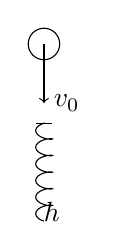
\begin{tikzpicture}
        \wall{(-1.5,0)}{(1,-.2)};
        \draw [decoration={aspect=.4, segment length=6, amplitude=3,coil},decorate,-|] (0,0) -- (0,1.25); %amplitude调整螺线管的直径，segment length调整间距
        \draw (0,2.25) circle (.2);
        \draw [->] (0,2.25) -- (0,1.5) node [right] {$v_0$};
        \length{(-.75,2.25)}{(-.75,0)}{$h$}{(0,-.5)};
    \end{tikzpicture}\vspace*{\fill}
\end{problem}
\end{paracol}
\begin{solution}
    整个过程中，小球所受合外力不为零，所以动量不守恒；有外力对小球做功，所以动能不守恒；小球和弹簧接触过程中机械能与弹簧的弹性势能发生相互转换，所以机械能不守恒.
\end{solution}

\begin{problem}
    2021年5月，我国首次火星探测任务天问一号探测器成功着陆火星. 是历史上第三个，也是唯一一个一次性实验``绕、落、巡''的国家. 为了实现大范围探测火星周围空间，天问一号轨道是一个巨大的椭圆. 已知火星中心在轨道的焦点上，火星半径为$R=\qty{3400}\km$，天问一号轨道近火点距火星表面$r_A=\qty{256}\km$，在轨道近火点处速度为$v_A=\qty{4.6}{\km/\s}$，远火点处距火星表面$r_B=\qty{11945.6}\km$，则在远火点处，天问一号速度大小为
    \begin{tasks}(4)
        \task $\qty{102}{\m/\s}$
        \task $\qty{207.4}{\km/\s}$
        \task $\qty{19.26}{\km/\s}$
        \task[\true] $\qty{1.10}{\km/\s}$
    \end{tasks}
\end{problem}
\solute1
\begin{solution}
    由探测器对火星角动量守恒$mv_A(R+r_A)=mv_B(R+r_B)$得远火点处速度$v_B=\qty{1.10}{\km/\s}$.
\end{solution}

\begin{paracol}{2}
\begin{problem}
    阿特伍德机是用于测量加速度及验证运动定律的机械，如图，考虑理想情况，滑轮质量、绳子质量及运动中的摩擦阻力都忽略不计，绳子不可伸长，物体$A$的质量$m_1$大于物体$B$的质量$m_2$，在$A$、$B$运动过程中弹簧秤$S$的读数是
    \begin{tasks}(4)
        \task $(m_1+m_2)g$
        \task $(m_1-m_2)g$
        \task[\true] $\frac{4m_1m_2}{m_1+m_2}g$
        \task $\frac{2m_1m_2}{m_1+m_2}g$
    \end{tasks}
    \switchcolumn\vspace*{\fill}\centering
    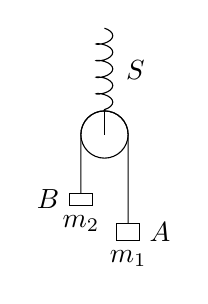
\begin{tikzpicture}[scale=.75]
        \wall{(1,1.8)}{(-1,2)};
        \draw (0,0) circle (.4);
        \draw [decoration={aspect=.4, segment length=6, amplitude=3,coil},decorate] (0,1.8) -- (0,.4) node [midway,right=1ex] {$S$}; %amplitude调整螺线管的直径，segment length调整间距
        \draw (0,.4) -- (0,0);
        \draw (-.6,-1) rectangle (-.2,-1.2);
        \draw (.2,-1.5) rectangle (.6,-1.8);
        \draw (-.4,-1) -- (-.4,0) arc (180:0:.4) -- (.4,-1.5);
        \node [below] at (-.4,-1.2) {$m_2$} node [left] at (-.6,-1.1) {$B$};
        \node [below] at (.4,-1.8) {$m_1$} node [right] at (.6,-1.65) {$A$};
    \end{tikzpicture}\vspace*{\fill}
\end{problem}
\end{paracol}
\solute2
\begin{solution}
    由于$m_A>m_B$，以竖直向下为正方向. 二者加速度方向相反，大小均为$a=(m_1-m_2)g/(m_1+m_2)$. 设弹簧秤张力为$T$. 由质心运动定律，对$m_1$和$m_2$有$(m_1+m_2)g-T=(m_1-m_2)a$. 代入$a$表达式得弹簧秤$S$的读数是$4m_1m_2/(m_1+m_2)g$.
\end{solution}

\begin{problem}
    一长$l$，质量$2m$的船浮于静水中，一个质量也为$m$的人从船尾走到船头. 不计水和空气的阻力，则在此过程中船将
    \begin{tasks}(4)
        \task[\true] 后退$l/3$
        \task 后退$l/2$
        \task 后退$l$
        \task 不动
    \end{tasks}
\end{problem}
\solute2
\begin{solution}
    人船系统水平方向上动量守恒，质心位置不变. 设人在行走过程中船运动的距离为$x$，由于二者的位置变化对系统质心位置变化的贡献为零，所以有
    \[m(l+x)+2mx=0\]
    其中$l+x$为人相对地面的位移. 解得$x=-l/3$. 负号表示船与人的运动方向相反，即后退$l/3$.
\end{solution}

\begin{problem}
    正方形的两对角上，各置点电荷$Q$，在另两对角上各置点电荷$q$. 若$Q$所受合力为零，则$Q$与$q$的关系为
    \begin{tasks}(4)
        \task[\true] $Q=-2\sqrt2q$
        \task $Q=-\sqrt2q$
        \task $Q=-4q$
        \task $Q=-2q$
    \end{tasks}
\end{problem}
\begin{solution}
    由题意知$Q$与$q$异号，$Q$所受次近邻电荷$Q$的斥力与所受两个近邻电荷$q$的引力平衡，即$\sqrt2Qq/a^2=Q^2/(\sqrt2a)^2$，所以$Q$与$q$的关系为$Q=-2\sqrt2q$.
\end{solution}

\begin{problem}
    一质量为$m$的小球沿光滑水平面以速度$v$运动，与位于光滑水平面上质量为$M$的静止箱子上无质量的弹簧发生弹性碰撞，弹簧的劲度系数为$k$，则弹簧的最大压缩量是
    \begin{tasks}(4)
        \task[\true] $v\sqrt{mM/(m+M)k}$
        \task $v\sqrt{m/k}$
        \task $v\sqrt{(m+M)/k}$
        \task $v\sqrt{(m+M)^2/k}$
    \end{tasks}
\end{problem}
\solute1
\begin{solution}
    刚碰撞后$m$的速度大于$M$，弹簧不断压缩. 当$m$和$M$共速时，弹簧压缩量最大，弹性势能最大. 物块、弹簧、挡板组成的系统在水平方向上动量守恒和系统机械能守恒可分别列出
    \[\begin{dcases}
        mv_0=(m+M)v'\\
        \frac12mv_0^2=\frac12(m+M)v'^2+E_p
    \end{dcases}\]
    联立得弹簧的最大弹性势能为$E_p=mMv^2/2(m+M)$. 根据弹簧弹性势能表达式$E_p=k\Delta x^2/2$得弹簧的最大压缩量$\Delta x_{\max}=v\sqrt{mM/k(m+M)}$.
\end{solution}

\begin{paracol}{2}
\begin{problem}
    质量为$m$的质点，以不变速率$v$沿图中正方形$ABCD$的水平光滑轨道运动. 质点越过$A$角时，轨道作用于质点的冲量的大小为
    \begin{tasks}(4)
        \task $\sqrt2mv/2$
        \task[\true] $\sqrt2mv$
        \task $mv$
        \task $2\sqrt2mv$
    \end{tasks}
    \switchcolumn\vspace*{\fill}\centering
    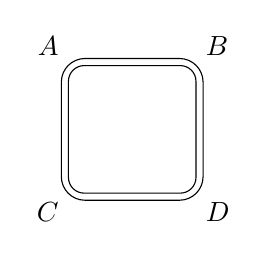
\begin{tikzpicture}[scale=.9]
        \draw [rounded corners=.3cm] (-1,1) rectangle (1,-1);
        \draw [rounded corners=.2cm,scale=.9] (-1,1) rectangle (1,-1);
        \node [above left] at (-.9,.9) {$A$};
        \node [above right] at (.9,.9) {$B$};
        \node [below left] at (-.9,-.9) {$C$};
        \node [below right] at (.9,-.9) {$D$};
    \end{tikzpicture}\vspace*{\fill}
\end{problem}
\switchcolumn
\begin{solution}
    $\abs{\Delta\bm p}=\abs{mv\bm i-(-mv\bm j)}=\sqrt2mv$.
\end{solution}
\end{paracol}

\begin{paracol}{2}
\begin{problem}
    一均匀静电场，电场强度$\bm E=(400\bm i+600\bm j)\unit{\V/\m}$，则通过如图阴影表面的电场强度通量是多少（正方体边长为$\qty1\cm$）
    \begin{tasks}(4)
        \task $\qty{0.01}{\V\cdot\m}$
        \task $\qty{0.02}{\V\cdot\m}$
        \task[\true] $\qty{0.04}{\V\cdot\m}$
        \task $\qty{0.06}{\V\cdot\m}$
    \end{tasks}
    \switchcolumn\vspace*{\fill}\centering
        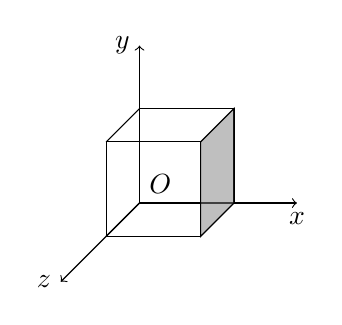
\begin{tikzpicture}
            \draw [->] (0,0) node [above right] {$O$} -- (0,2) node [left] {$y$};
            \draw [->] (0,0) -- (2,0) node [below] {$x$};
            \draw [->] (0,0) -- (-1,-1) node [left] {$z$};
            \begin{scope}[xshift=-1cm]
                \draw (1,0) rectangle (2.2,1.2);
                \draw [xshift=-.3*sqrt(2)*1cm,yshift=-.3*sqrt(2)*1cm] (1,0) rectangle (2.2,1.2);
                \draw ({1-.3*sqrt(2)},{-.3*sqrt(2)}) -- (1,0) ({1-.3*sqrt(2)},{1.2-.3*sqrt(2)}) -- (1,1.2);
                \filldraw [fill=gray,fill opacity=.5] ({2.2-.3*sqrt(2)},{1.2-.3*sqrt(2)}) -- (2.2,1.2) -- (2.2,0) -- ({2.2-.3*sqrt(2)},{-.3*sqrt(2)}) -- cycle;
            \end{scope}
        \end{tikzpicture}\vspace*{\fill}
\end{problem}
\switchcolumn
\solute0
\begin{solution}
    $\Phi=\oiint\bm E\cdot\d\bm S=400\times(\num{1e-2})^2=\qty{0.04}{\V\cdot\m}$.
\end{solution}
\end{paracol}

\begin{paracol}{2}
\begin{problem}
    如图所示，一球对称性静电场的电场强度与径向距离的关系曲线，请指出该电场是由下列哪种带电体产生的
    \begin{tasks}(4)
        \task 点电荷
        \task* 内外半径分别为$r$和$R$均匀带电厚球壳
        \task*(2) 半径为$R$均匀带电薄球壳
        \task*(2)[\true] 半径为$R$均匀带电球体
    \end{tasks}
    \switchcolumn\vspace*{\fill}\centering
    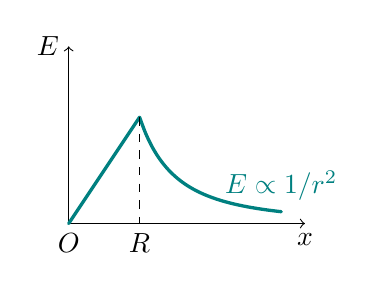
\begin{tikzpicture}[scale=1.5]
        \draw [<->] (0,1.5) node [left] {$E$} -- (0,0) node [below] {$O$} -- (2,0) node [below] {$x$};
        \draw [very thick,teal,variable=\x,domain=0:.6,smooth,line cap=round] plot ({\x},{1.5*\x});
        \draw [very thick,teal,variable=\x,domain=.6:1.8,smooth,line cap=round] plot ({\x},{.324/\x/\x}) node [above] {$E\propto1/r^2$};
        \draw [dashed] (.6,.9) -- (.6,0) node [below] {$R$};
    \end{tikzpicture}\vspace*{\fill}
\end{problem}
\end{paracol}

\begin{problem}
    一点电荷，放在球形高斯面的中心处. 下列哪一种情况，通过高斯面的电场强度通量发生变化
    \begin{tasks}(2)
        \task 将另一点电荷放在高斯面外
        \task[\true] 将另一点电荷放进高斯面内
        \task 将球心处的点电荷移开，但仍在高斯面内.
        \task 将高斯面半径缩小
    \end{tasks}
\end{problem}
\begin{solution}
    由高斯定理，通过高斯面的电场强度通量只与其内部电荷量有关.
\end{solution}

\section{填空题（共18分）}

\begin{problem}
    质量为$m$的小球自高为$y_0$处沿水平方向以速率$v_0$抛出，与地面碰撞后跳起的最大高度为$y_0/2$，水平速率为$v_0/2$，则碰撞过程中
    \begin{enumerate}
        \item 地面对小球的竖直冲量的大小为\ans{$m\ab(\sqrt{2gy_0}+\sqrt{gy_0})$}.
        \item 地面对小球的水平冲量的大小为\ans{$mv_0/2$}.
    \end{enumerate}
\end{problem}
\solute1
\begin{solution}
    碰撞前后，小球竖直方向速度大小分别为$\sqrt{2gy_0}$和$-\sqrt{2gy_0/2}$，由动量定理得地面对小球的竖直冲量的大小为$m\ab(\sqrt{2gy_0}+\sqrt{gy_0})$，地面对小球的水平冲量的大小为$mv_0-mv_0/2=mv_0/2$.
\end{solution}

\begin{paracol}{2}
\begin{problem} % {转动定律，圆周运动}
    如图所示，一质量为$m$、半径为$R$的薄圆盘，可绕通过其一直径的光滑固定轴$AA'$转动，转动惯量$I=mR^2/4$.该圆盘从静止开始在恒力矩$M$作用下转动，$t$秒后位于圆盘边缘上与轴$AA'$的垂直距离为$R$的$B$点的法向加速度$a_n=$\ans{$16M^2t^2/m^2R^3$}.
    \switchcolumn\vspace*{\fill}\centering
    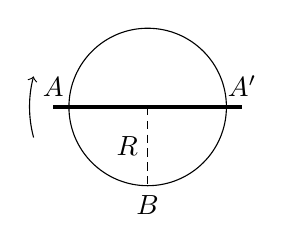
\begin{tikzpicture}
        \draw (0,0) circle (1);
        \draw [very thick] (-1.2,0) node [above] {$A$} -- (1.2,0) node [above] {$A'$};
        \draw [densely dashed] (0,0) -- (0,-1) node [midway,left] {$R$} node [below] {$B$};
        \draw [->] ({-1.5*cos(15)},{-1.5*sin(15)}) arc (195:165:1.5);
    \end{tikzpicture}\vspace*{\fill}
\end{problem}
\end{paracol}
\begin{solution}
    圆盘的角加速度$\beta=M/I=4M/mR^2$. $t$秒后圆盘的角速度$\omega=\beta t=4Mt/mR^2$，$B$点的法向加速度为$a_n=\omega^2R=16M^2t^2/m^2R^3$.
\end{solution}

\begin{problem}
    一颗速率为$\qty{700}{\m/\s}$得子弹，打穿一块木板后速率降到$\qty{500}{\m/\s}$. 如果让它继续穿过厚度和阻力均与第一块完全相同的第二块木板，则子弹的速率将降到\ans{$\qty{100}{\m/s}$}.
\end{problem}
\solute0
\begin{solution}
    由题意知两次阻力做功相同，根据动能定理得两次$v^2$的变化量相同. 所以穿过第二块木板后子弹的速率降到$v=\sqrt{500^2-(700^2-500^2)}=\qty{100}{\m/\s}$.
\end{solution}

\begin{paracol}{2}
\begin{problem}
    $A$、$B$为真空中两个平行的``无限大''均匀带电平面，$A$板带负电荷，$B$板带正电荷. 已知两平面间的电场强度大小为$E_0$，两平面外侧电场强度大小都为$E_0/2$，方向如图. 则$A$，$B$两平面上的电荷面密度分别为$\sigma_A=$\ans{$-\epsilon_0E_0/2$}，$\sigma_B=$\ans{$3\epsilon_0E_0/2$}.
    \switchcolumn\centering
    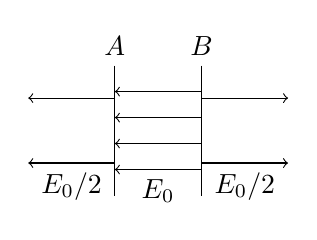
\begin{tikzpicture}[scale=.55]
        \draw (-1,1.5) node [above] {$A$} -- (-1,-1.5);
        \draw (1,1.5) node [above] {$B$} -- (1,-1.5);
        \draw [->] (-1,.75) -- (-3,.75);
        \draw [->] (-1,-.75) -- (-3,-.75) node [midway,below] {$E_0/2$};
        \draw [<-] (-1,-.9) -- (1,-.9) node [midway,below] {$E_0$};
        \draw [<-] (-1,-.3) -- (1,-.3);
        \draw [<-] (-1,.3) -- (1,.3);
        \draw [<-] (-1,.9) -- (1,.9);
        \draw [->] (1,.75) -- (3,.75);
        \draw [->] (1,-.75) -- (3,-.75) node [midway,below] {$E_0/2$};
    \end{tikzpicture}
\end{problem}
\end{paracol}
\solute1
\begin{solution}
    由无限大带电平面附近的场强表达式$E_0=\sigma/2\epsilon_0$，左（右）侧和中间区域场强满足
    \[\frac{\sigma_A}{2\epsilon_0}+\frac{\sigma_B}{2\epsilon_0}=\frac{E_0}{2},\ \frac{\sigma_B}{2\epsilon_0}-\frac{\sigma_A}{2\epsilon_0}=E_0\]
    解得$\sigma_A=-\epsilon_0E_0/2$，$\sigma_B=3\epsilon_0E_0/2$.
\end{solution}

\section{计算题（共46分）}

\begin{problem}
    1984年4月8日，我国第一颗地球同步通信卫星``东方红二号''成功发，使新疆乌鲁木齐市从此能直接受到中央电视台当天播出的电视节目，``海内存知己，天涯若比邻''的诗情画意成为美好的现实. 地球静止同步卫星轨道是一个与地球赤道同心共面的圆，从固定在地球上的观察者看来，卫星保持静止不动. 试求卫星的轨道离地面的高度为多少？（卫星在轨道上运行的方向与地球自转方向相同，地球自转一周所需时间为$24$小时，地球半径为$\qty{6.4e6}\m$，地球质量为$\qty{5.97e24}\kg$，万有引力常量$G=\qty{6.67e-11}{\m^3\cdot\kg^{-1}\cdot\s^{-2}}$）.
\end{problem}
\solute0
\begin{solution}
    地球自转角速度$\omega=2\pi/T=\qty{7.27e-5}{\radian/\s}$. 由万有引力提供卫星做圆周运动时的向心力
    \[m\omega^2(R+h)=\frac{GMm}{(R+h)^2}\]
    得卫星的轨道离地面的高度为$h=\sqrt[3]{GM/\omega^2}-R=\qty{3.58e7}\m$.
\end{solution}

\begin{problem}
    鸟山明先生是世界著名漫画家，曾借「龙珠」角色之口公开反战反侵略，在作品中传达爱与和平的精神. 我国外交部也对他的逝世表达深切哀悼和诚挚慰问. 亀派气功是鸟山明作品「龙珠」中的主角孙悟空常使用的绝招，使用时将双手合成花萼状，在手掌心汇聚出一个能量球，将能量以的速度发射出去攻击对手.

    假设能量球发射时的初速度$v_0=\qty{1000}{\m/\s}$，飞行时，速度会随飞行距离逐渐减小，满足$\odv v/x=-\alpha v$，其中衰减系数$\alpha=\qty{0.02}{/\m}$. 假设当能量球速度下降到$v _x=\qty{1}{\m/\s}$时，人类能够承受其攻击，则亀派气功的杀伤范围为多大？（$\ln0.001\approx-6.908$）.
\end{problem}
\solute4
\begin{solution}\leavevmode
    \begin{itemize}
        \item 将能量球速度随飞行距离的微分方程分离变量$\d v/v=-\alpha\d x$，对其积分得$\ln v=-\alpha x+C$.
        \item 由初始条件$x=0$，$v=v_0$得常数$C=\ln v_0$. 所以能量球速度随飞行距离的关系式为$v=v_0\e^{-\alpha x}$.
        \item 由题意，人类能够承受其能量球攻击的速度大小为$v'=\qty{1}{\m/s}$. 此时能量球的飞行距离为$x_0=\frac1\alpha\ln v_0/v'=\qty{345.39}\m$. 所以亀派气功的杀伤范围为$S=\pi x_0^2=\qty{3.75e5}{\m^2}$.
    \end{itemize}
\end{solution}

\begin{problem}
    一根放在水平光滑桌面上的匀质棒，可绕通过其一端的竖直固定光滑轴$O$转动. 棒的质量为$m=\qty{1.5}\kg$，长为$l=\qty{1.0}\m$，对轴的转动惯量为$I=ml^2/3$，初始时棒静止. 有一水平运动的子弹垂直射入棒的$A$端，并留在棒中. 子弹的质量为$m'=\qty{0.02}\kg$，速率为$v=\qty{400}{\m/\s}$. 试问
    \begin{enumerate}
        \item 棒开始和子弹一起转动时角速度$\omega$有多大？
        \item 若棒转动时受到大小为$M_r=\qty{4.0}{\N\cdot\m}$的恒定阻力矩作用，棒能转过多大的角度$\theta$？
    \end{enumerate}
\end{problem}
\solute0
\begin{solution}\leavevmode
    \begin{enumerate}
        \item 由子弹和棒组成的系统对$O$点角动量守恒$m'v_0l=(ml^2/3+m'l^2)\omega$得入射后棒的角速度$\omega=3m'v_0/(3m'+m)l=\qty{15.38}{\radian/\s}$.
        \item 由动能定理$M_r\theta=\frac12(ml^2/3+m'l^2)\omega^2$得棒能转过的角度$\theta=\qty{15.38}{\radian}$.
    \end{enumerate}
\end{solution}

\begin{problem} % {动量守恒}
    一电子和一个静止着的氢原子发生对心完全弹性碰撞. 已知氢原子质量为电子质量的$1840$倍，求碰撞过程中传给氢原子的能量与电子原来能量的比值.
\end{problem}
\solute0
\begin{solution}
    设电子质量为$m$，氢原子质量为$1840m$，电子速率为$v_0$. 碰撞过程中氢原子和电子组成的系统动量守恒
    \[mv_0=mv_1+1840mv_2\]
    由于碰撞为完全弹性碰撞，所以碰撞过程中能量守恒
    \[\frac12mv_0^2=\frac12mv_1^2+\frac12\cdot 1840 mv_2^2\]
    联立以上两式得$\Delta E_k/E_{k_0}=1840v_2^2/v_0^2=\num{2.17e-3}$.
\end{solution}

\begin{problem}
    两个无限长同轴柱圆柱面，半径分别为$R_1$，$R_2$（$R_2>R_1$）带有等值异号电荷，每单位长度的电量为$\lambda$，试求
    \begin{tasks}[label=\arabic*.](2)
        \task $r>R_2$时离轴线为$r$处的电场强度.
        \task $R_1<r<R_2$时离轴线为$r$处的电场强度.
    \end{tasks}
\end{problem}
\begin{solution}\leavevmode
    \begin{enumerate}
        \item 取半径$r>R_2$，高度为$l$的圆柱高斯面，由高斯定理$E_1\cdot 2\pi rl=[+\lambda l+\ab(-\lambda)l]/\epsilon_0$得$E_1=0$.
        \item 取半径$R_1<r<R_2$，高度为$l$的圆柱高斯面，由高斯定理$E_2\cdot 2\pi rl=\lambda l/\epsilon_0$得$E_2=\lambda/2\pi r\epsilon_0$.
    \end{enumerate}
\end{solution}

\begin{problem}
    一不可伸长的轻绳一段系一个质量为$m$的小球，绳子另一端穿过光滑水平桌面上一个小孔，并有一拉力作用其上. 绳子与小孔之间摩擦力忽略不计，小球以角速度$\omega$做半径为$R$的匀速圆周运动. 当拉力作用下小球圆周运动半径变为$r$时，拉力做功多少？
\end{problem}
\solute0
\begin{solution}\leavevmode
    \begin{itemize}
        \item 由拉拽绳子过程中小球对小孔的角动量守恒$mR^2\omega=mr^2\omega'$得$\omega'=\omega R^2/r^2$.
        \item 由动能定理得$W=\frac12mr^2\omega'^2-\frac12mR^2\omega^2=\frac12mR^2\omega^2(R^2/r^2-1)$.
    \end{itemize}
\end{solution}